
\section{Equipo de a bordo}

Cuatro son los componentes del equipo de a bordo del sistema VOR. Estos son:

\begin{itemize}
\item Antena 

\item Receptor


\item Servoamplificador 

\item Indicador

\end{itemize}

\subsection{Antena }

La antena del equipo VOR no tiene complicación alguna y tan solo cabe destacar su forma en V y que, casi siempre, va instalada en el estabilizador vertical de cola o en la parte superior del fuselaje. Su misión consiste en recibir las líneas de flujo electromagnético emitidas por la estación de tierra y transmitirlas al receptor.

\subsection{Receptor }

La función del receptor consiste en interpretar o medir, con ayuda de los indicadores, la diferencia de fase entre las dos señales la de referencia y la  variable, emitidas por el equipo de tierra. Los modernos receptores suelen tener los siguientes mandos de control:

\subsubsection{On/off-volumen}
Cuando este interruptor está en su posición OFF, el receptor no recibe energía, y  por tanto, permanece inactivo. Cuando su posición es ON, está ya preparado para su funcionamiento. Si se sigue girando este interruptor cuando está en ON, el  resultado es un aumento de volumen en la recepción de la estación selectada. Este mando de volumen no afecta, aunque esté en su posición de mínimo, a la señal de navegación que Ilega al indicador.

\subsubsection{Selector de frecuencias}
Consiste en dos ruedas con las que se selectan las frecuencias. Una de ellas selecciona las comprendidas entre 108 y 136 Mhz, y la otra selecciona Khz o centésimas de Mhz. Este selector permitirá, pues, selectan un canal entre 560 posibles.

Aunque el emisor del equipo VOR trabaja casi siempre entre 112 y 118 Mhz, el receptor de a borde cubre la banda comprendida entre 108 y 136 Mhz, con lo que es capaz de admitir frecuencias para operar en las funciones ILS, VOR y comunicaciones en radiotelefonía aire - tierra y tierra-aire. La banda de frecuencias que se puede sintonizar en el receptor tiene la siguiente distribución:

\begin{itemize}
\item De 108 Mhz a 112 Mhz, para ILS y VOR 

\item De 112 Mhz a 117,9 Mhz, para VOR.

\item De 118 Mhz a 135,9 Mhz, para radiotelefonía

\end{itemize}

El motivo de que el receptor sea capaz de cubrir las tres funciones mencionadas, radica en la necesidad de condensar al máximo el equipo de cabina. De esta manera se evita el tener que instalar un receptor independiente para cada equipo.

\subsubsection{Ventanilla selectora}
En ella se lee la frecuencia selectada.

\subsubsection{Interruptor filtro de identificación (Ident)}
El tono de identificación de la estación de tierra es filtrado, mediante la presión del interruptor IDENT, cuando es muy necesaria una recepción nítida y clara de dicho tono.

\begin{figure}[!hb]
  \centering
  \subfigure[Antena recepción señales VOR]{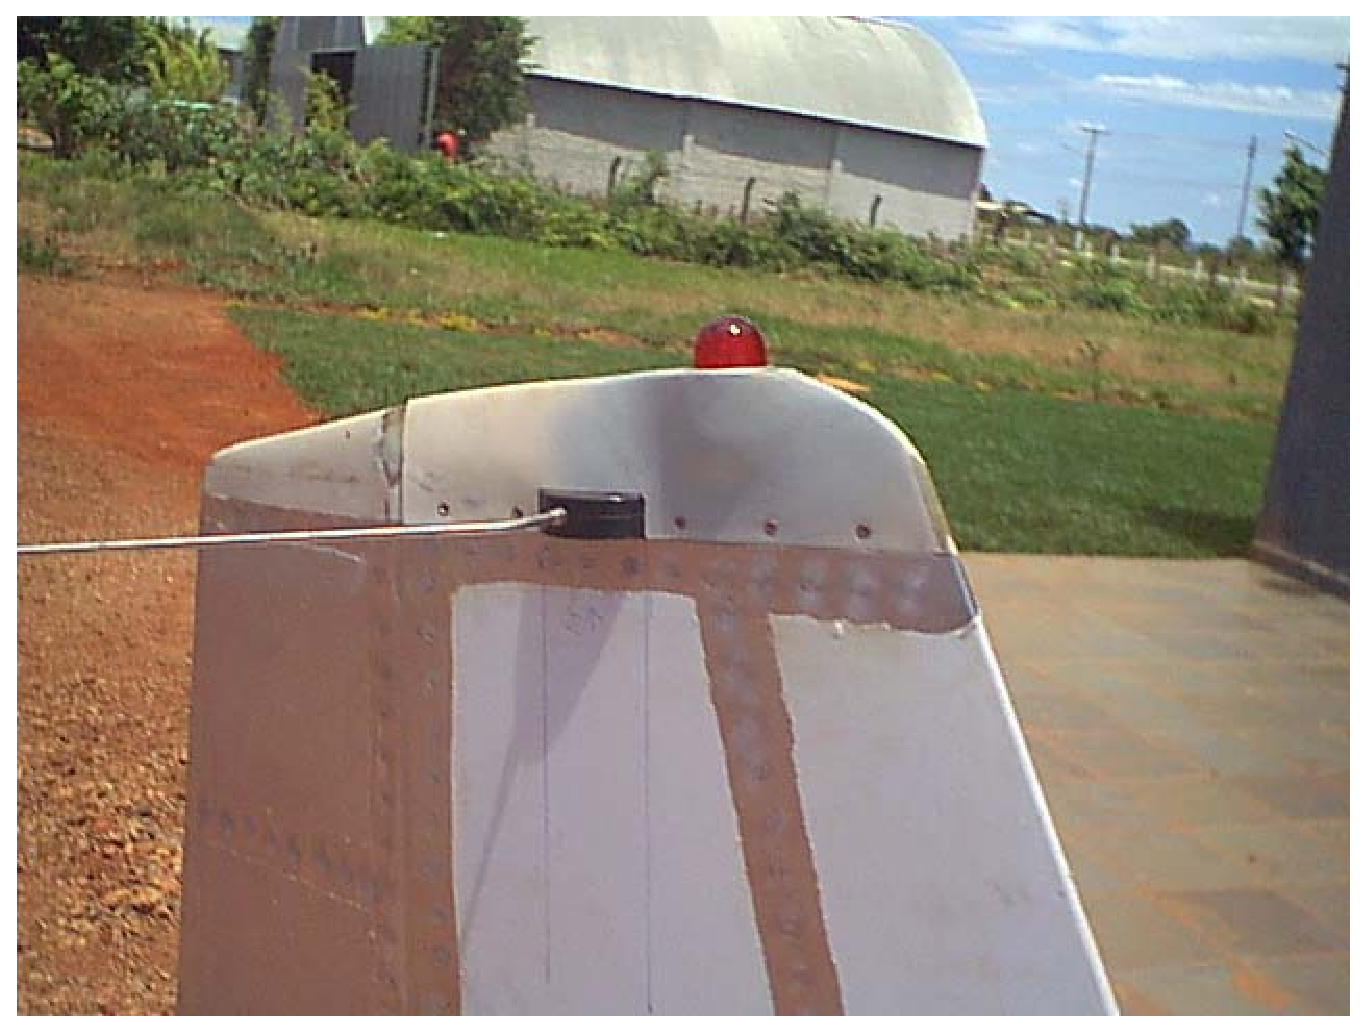
\includegraphics[width=0.3\textwidth]{Imagenes/06.02.vor.imagenes/Antena_Vor_empenaje_vertical.eps}}
  \subfigure[Receptor (Nav-Com)]{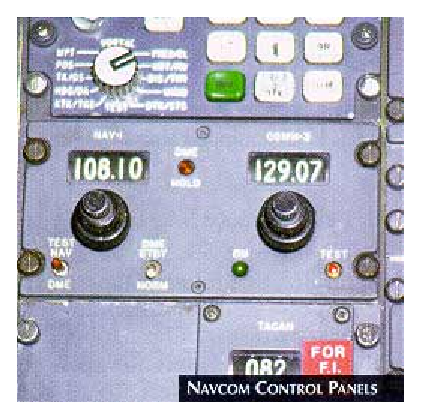
\includegraphics[width=0.3\textwidth]{Imagenes/06.02.vor.imagenes/Nav-com.eps}}
  \subfigure[Indicador VOR (modelo obsoleto!)]{
\includegraphics[width=0.3\textwidth]{Imagenes/06.02.vor.imagenes/Indicador-vor-viejo.eps}}
  \caption{Equipo a bordo sistema VOR}
\end{figure}


\subsection{Servoamplificador}
La energía electromagnética llega desde el emisor de tierra hasta la antena de a bordo. Desde allí es enviada al receptor, donde es convertida en impulsos eléctricos. Estos impulsos no bastarán para producir las deflexiones necesarias en indicador VOR, por lo que tienen que ser tratados por un servoamplificador. Una vez amplificados los impulsos ya pueden ser transmitidos al indicador.

\subsection{Indicador VOR}

La función única del indicador VOR, es mostrar al piloto su situación con respecto a la estación de tierra en cualquier momento. La información es clara y precisa y da, constantemente, indicaciones de mando, o da qué debe hacer el piloto para mantener a la aeronave sobre una ruta determinada. 

\begin{figure}[!htb]
  \centering
  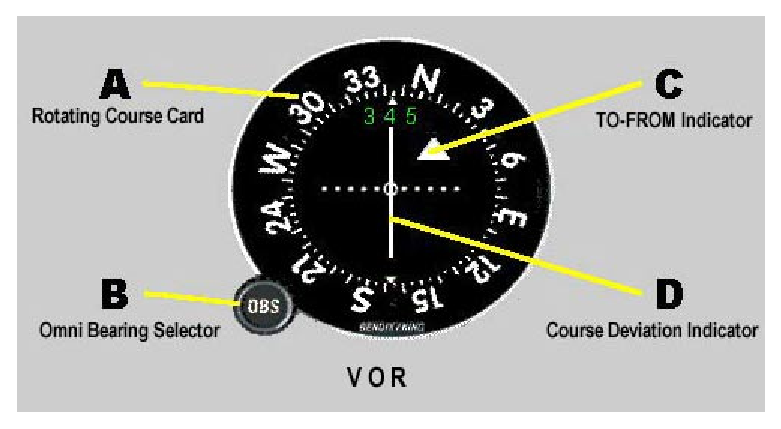
\includegraphics[width=\textwidth]{Imagenes/06.02.vor.imagenes/vor_indicator.eps}
  \caption{Partes de un indicador VOR}
  \label{fig:indicador-vor}
\end{figure}

Aunque hay muchos tipos de indicadores VOR, este estudio se ce\~nir\'a a la descripci\'on de un equipo moderno que consta de los siguientes elementos:

\begin{itemize}

\item \textbf{Selector de rutas (OBS):} Con el OBS (Omni - Bearing Selector), el piloto puede seleccionar la ruta que desee con el fin de interceptarla y acercarse o alejarse por ella, de una estación VOR. El OBS es un pequeño mando adosado a la caja del instrumento, y con él se gobierna la rotación de la carta o rosa graduada en 360 grados que va instalada en el interior del indicador VOR.


\item \textbf{Bandera TO-0FF-FROM:} La misión de la bandera TO - OFF - FROM, es resolver los 180 grados de ambigüedad que tendría la ruta seleccionada, mostrando si ésta, una vez haya sido interceptada, conducirá al avión hacia (TO) la estación, o por el contrario, si le alejará de ella (FROM). Si la aeronave está fuera del alcance de la estación de tierra, y por tanto no recibe una señal fiable, el indicador  TO - FROM desaparecerá, siendo sustituido por la palabra OFF. Este indicador será también visible cuando la aeronave se encuentre en el cono de silencio de la estación VOR, o cuando la ruta seleccionada se encuentre entre 85 grados ó 90 grados de distancia de la posición real del avión. La banderilla TO - OFF - FROM es activada por medio de energía eléctrica procedente de las fuentes principales del avión (corriente continua).


\item \textbf{Indicador de desvío de ruta (CDI):} Una vez una ruta haya sido selectada e interceptada, el CDI (Course Desviatìon Indicator), indicará al piloto si la está siguiendo correctamente, o si por el contrario se ha desviado de ella. Si el avión está sobre la ruta seleccionada, al CDI estará centrado en el instrumento. El piloto puede pensar en el CDI como en un pedacito de ruta trasladado a su indicador de a bordo. Considerándolo de esta manera, cuando el avión se encuentre a la derecha de la ruta seleccionada, el CDI estará desplazado a la izquierda del instrumento. En el caso opuesto, cuando e1 avión esté volando a la izquierda de la ruta, el CDI estará desplazado a la derecha del instrumento. En cualquier caso, el CDI indicará a qué lado del avión está la ruta que el piloto haya seleccionado y hacia dónde tiene éste que virar para reinterceptarla. En el centro del instrumento y en cada una de sus mitades, hay dibujados cinco puntos que indican la distancia en grados entre la ruta seleccionada y el avión. Un desplazamiento del CDI de dos puntos, indicará una separación de cuatro grados. Cada punto equivale, pues, a dos grados. Es evidente que el haz que cubre el instrumento en cada lado de la ruta seleccionada, es de diez grados.

\item \textbf{Pulsador de TEST:} Sirve única y exclusivamente para medir la seguridad de las indicaciones del CDI. Haciendo uso del pulsador, el CDI sufrirá un desplazamiento determinado hacia uno de los lados del instrumento, lo cual indicará su buen funcionamiento. En caso de que el CDI no reaccionara de esta manera, eI instrumento no sería de fiar. En muchos instrumentos eI TEST va instalado en el mismo mando que el OBS.

\item \textbf{Fiel:} El fiel es un punto grabado en la parte superior de la caja del instrumento, bajo el cual, el piloto situará la ruta deseada.

\item \textbf{Fiel de ruta reciproca:} Este fiel es diametralmente opuesto al anterior, y sirve al piloto como recordatorio de la ruta recíproca a la que lleva selectada.

\item \textbf{Referencias de 90 grados:} Son otros dos puntos situados a derecha e izquierda del indicador, dando referencia de cuáles son las rutas situadas a 90 grados de la ruta seleccionada.


\end{itemize}